\section{Materiali e metodi}

In questa sezione verranno presentati i materiali e i metodi utilizzati in questo lavoro. Come primo elemento verrà introdotto il dataset utilizzato. Successivamente, verranno presentati i metodi di preprocessing dei segnali fisiologici considerati e come si è ovviato al problema della loro asincronicità durante l'estrazione delle feature.
Verrà illustrato il processo di selezione delle feature estratte, per conservare quelle più efficaci alla classificazione delle emozioni.
In ultimo, verrà presentato il modello delle mappe di salienza fisiologiche e il loro impiego nel processo di video summarization.

\subsection{Dataset}

Lo studio utilizza i dati contenuti in MAHNOB-HCI \cite{soleymani2011multimodal}: un database, disponibile online, che fornisce campionamenti di segnali fisiologici, e valori di self-report, in risposta alla sollecitazione emotiva di un soggetto.

Alla raccolta dei dati hanno partecipato 16 femmine e 11 maschi, con differenti backgroud culturali.

L'intero database contiene dati relativi a due diversi setup sperimentali:

\begin{enumerate}
    \item Emotion recognition: in cui ai partecipanti è stato chiesto di guardare 20 clip video, estratte da film e show televisivi, con lo scopo di indurre una risposta emotiva. Le clip sono scelte a caso da un insieme più ampio e prima di ogni clip, è stato mostrata una piccola clip neutrale, al fine di ridurre il bias dovuto allo stato emotivo del soggetto.
    Al termine di ogni clip, i soggetti hanno compilato, utilizzando i valori da 1 a 9 di un tastierino numerico, il questionario di self-reporting per annotare la propria risposta emotiva in termini di:
    \begin{itemize}
        \item Emozione percepita, \emph{feltEmo}, la codifica numerica è riportata in tabella~\ref{tab:emotions_map}.
        \item Arousal percepito, \emph{feltArsl}: 1 per nessuna attivazione, 9 per massima attivazione.
        \item Valence percepito, \emph{feltVlnc}: 1 per molto negativo, 9 per molto positivo, 5 per neutrale.
        \item Control percepito, \emph{feltCtrl}: 1 per senza controllo, 9 per pieno controllo.
        \item Predictability percepita, \emph{feltPred}: 1 per imprevedibile, 9 per completamente prevedibile.
    \end{itemize}
    questi valori, insieme ad altri, sono riportati nel file di metadati associato ad ogni sessione.

    \item Implicit tagging: che prevede di mostrare una sequenza di clip video o immagini, prima senza tag e successivamente con un tag che descriva, talvolta in modo corretto talvolta in modo errato, l'emozione che questa rappresenta. Ai partecipanti è stato chiesto di annotare se fossero in accordo o in disaccordo con la descrizione dell'emozione indicata.
\end{enumerate}

\begin{table}[]
\centering
\begin{tabular}{c|c}
\toprule
Codifica Numerica & Nome Emozione \\
\midrule
0                 & Neutrale \\
1                 & Rabbia \\
2                 & Disgusto \\
3                 & Paura \\
4                 & Gioa, felicità \\
5                 & Tristezza \\
6                 & Sorpresa \\
11                & Divertimento \\
12                & Ansia \\
\bottomrule
\end{tabular}
\caption{Codifica numerica delle emozioni selezionabili nei questionari di self-report.}
\label{tab:emotions_map}
\end{table}

Le sessioni sperimentali sono state successivamente suddivise per singolo stimolo, catalogate e identificate univocamente da un file XML contenente i relativi metadata. Il file descrive il contenuto della singola sessione, indicandone i riferimenti a soggetto partecipante, tipo di esperimento, lo stimolo mostrato, i valori del questionario di self-report e i riferimenti temporali per la gestione dei segnali fisiologici.

Il database include 6 registrazioni video del soggetto riprese da angolature diverse, 2 segnali audio, dati di eye-tracking e segnali fisiologici del sistema centrale e periferico, tra cui: 32 canali di EEG, 3 canali ECG, temperatura corporea e conduttanza cutanea.

\begin{table}[]
\centering
\begin{tabular}{lrrrrrrrr}
\toprule
{}         & N            & emo*   & \multicolumn{2}{l}{feltEmo} & \multicolumn{2}{l}{feltVlnc} & \multicolumn{2}{l}{feltArsl} \\
{}         & sessioni     & {}     &     mean &   std &     mean &   std &    mean &   std  \\
Media                     &        &          &       &          &       &         &        \\
\midrule
30         & 25           & 3      &     5.56 &  3.84 &     2.84 &  1.70 &    6.36 &  1.70  \\
53         & 18           & 11     &     7.71 &  4.55 &     4.38 &  2.04 &    5.62 &  1.47  \\
69         & 26           & 2      &     3.19 &  3.25 &     2.23 &  1.07 &    5.73 &  2.01  \\
90         & 26           & 4      &     7.92 &  4.07 &     6.76 &  1.39 &    4.16 &  1.99  \\
111        & 24           & 5      &     4.62 &  1.31 &     2.12 &  0.99 &    6.00 &  1.47  \\
\hline
Totale sessioni & 124   & & & & & & \\
\bottomrule
\end{tabular}
\caption{Media clip utilizzate durante i test di video summarization. Vengono indicati il numero di sessioni afferenti al singolo media, la classe di emozione a cui appartiene la clip (emo*) e il valore medio e deviazione standard delle valutazioni dei soggetti in termini di emozione provata (feltEmo), valence (feltVlnc), arousal (feltArsl).}
\label{tab:used_media}
\end{table}

In questo studio sono stati considerate 124 sessioni afferenti ai media riportati in tabella~\ref{tab:used_media}, in quanto rappresentativi delle differenti classi di emozioni. La tabella riassume il numero di sessioni per clip video, con relativo valore medio e deviazione standard delle risposte dei partecipanti.

Gli stimoli video utilizzati durano tra i 34.9 e i 117s $(M=81.4s; SD=22.5s)$, hanno una risoluzione di 1280x800 pixel e frame rate non omogeneo. Per ridurre i tempi computazionali, le clip selezionate sono state scalate a una risoluzione di 320x200 pixel con un framerate costante di 24pfs.

\subsection{Segnali fisiologici e feature}

Tra i diversi segnali fisiologici presenti nel dataset, in questo lavoro vengono utilizzati: gaze, ECG, EDA, SKT e Resp.
I dati di gaze sono campionati a 60Hz mentre i restanti segnali stato stati campionati a 1024Hz e successivamente sottocampionati a 256Hz per ridurre i tempi computazionali. Per il denoising e il preprocessing di ECG, SKT e Resp è stato utilizzato il toolbox per l'elaborazione di segnali biologici \emph{BioSPPy}\cite{carreiras2018biosppy}.

Al termine di tutte le elaborazioni, ai segnali risultanti è stato applicato un algoritmo di resampling per ottenere serie temporali a 24 sample/s.

Le caratteristiche principali e i trattamenti specifici dei segnali utilizzati sono di seguito descritti.

\subsubsection{Gaze}
I dati sono forniti dal gaze tracker Tobii X1205 in formato CSV. Il sistema fornisce un insieme di informazioni tra cui le coordinate del punto osservato dal partecipante, proiettate nello spazio coordinate dello schermo. Per ogni campione è fornito un codice di affidabilità della lettura del singolo occhio, la tabella \ref{tab:gaze_validity_values} fornisce la descrizione di ogni valore. Sulla base di questo codice è possibile estrarre i momenti in cui il partecipante chiude gli occhi, o $blink$. Le letture con affidabilità $>1$ sono considerate all'interno di un blink. Queste porzioni di segnale sono corrette con una interpolazione tra le coordinate dell'ultima misurazione valida e la prima successiva al blink. Dall'insieme dei dati forniti dal tracker sono stati letti e processati: le coordinate delle fissazioni e la loro durata, la distanza istantanea dell'occhio dal tracker e la media della dimensione della pupilla tra occhio sinistro e occhio destro.

La dimensione della pupilla è considerata come feature e non ha subito ulteriori elaborazioni.

\begin{table}[]
\begin{tabular}{p{0.1\textwidth}|p{0.8\textwidth}}
\toprule
Codice validità   & Descrizione \\
\midrule
0            & Il sistema è certo di aver registrato tutti i dati rilevanti di un particolare occhio
               e non c'è rischio di confondere occhio sinistro e occhio destro \\

1            & Il sistema ha registrato un occhio e ha fatto una assunzione,
               molto probabile, sul fatto che sia l'occhio sinistro o quello destro.
               In questo caso, il codice di validità dell'altro occhio è sempre 3 \\

2            & Il sistema ha registrato solo un occhio e non è in grado di stabilire quel sia \\

3            & Il sistema è confidente che il valore letto non è corretto o è corrotto.
               L'altro occhio ha sempre codice di validità 1 \\

4            & Il dato ottenuto è corrotto.  \\
\bottomrule
\end{tabular}
\caption{Codici di validità di ogni lettura del gaze tracker}
\label{tab:gaze_validity_values}
\end{table}

\subsubsection{ECG}
\uppercase{è} stato registrato usando tre sensori posizionati sul petto del partecipante. Il segnale è misurato in microvolt ($\mu$V).
Il primo step di elaborazione è l'applicazione un filtro bassa-banda con banda passante 3-45Hz per sopprimere rumore e interferenze.
Il secondo step prevede la ricerca degli \emph{R-peak} all'interno dei complessi QRS. Il tempo che intercorre tra due R-peak è definito come intervallo RR. Il reciproco di RR, moltiplicato per 60, fornisce una misura dei battiti per minuto (bpm) e quindi del heart rate (HR), secondo la relazione:
\begin{equation}
    HR(bpm) = \frac{60}{RR(s)}
\end{equation}
L'HR tipico di una persona a riposo può variare tra i 60 e i 100bpm.
Il segnale così ottenuto è stato poi utilizzato nelle fasi successive del lavoro

\subsubsection{EDA}
Viene misurata applicando due elettrodi alle falangi distali dell'indice e del medio. Fornisce una misura della resistenza della pelle al passaggio di corrente lungo il corpo, con voltaggio trascurabile ed e misurato in Ohm. La resistenza diminuisce all'aumentare della traspirazione, che generalmente avviene quando un soggetto è in condizioni di stress o prova emozioni di sorpresa. In \cite{lang1993looking} viene provata la relazione tra il valore medio di EDA e il livello di arousal.
Il segnale raw viene elaborato con un filtro passa-basso di quarto ordine e frequenza di taglio 5Hz. Al segnale viene applicata poi una funzione di smoothing, implementata come convoluzione di una funzione kernel boxzen e dimesione $s = \lfloor0.75 * fps\rfloor$.
Il segnale così ottenuto viene applicata una normalizzazione e si estrae la componente fasica usando l'algoritmo di convex optimization cvxEDA\cite{greco2015cvxeda}.

\subsubsection{Resp}
Viene ottenuto posizionando la cintura con il sensore di misurazione attorno all'addome del partecipante. Il segnale è misurato in $\mu$V. Il segnale raw viene elaborato applicando un filtro passa-banda con frequenze di taglio 0.1Hz e 0.35Hz, il segnale così ottenuto è stato poi utilizzato nelle fasi successive del lavoro.

\subsubsection{SKT}
Viene ottenuto applicando il sensore di misurazione sul mignolo del partecipante. Il segnale è misurato in Celsius. Il segnale raw è stato elaborato applicando un filtro bassa-passo di secondo ordine con frequenze di taglio 1Hz \cite{palanisamy2013multiple}. Il segnale filtrato è stato usato nelle fase successive del lavoro.

\subsection{Aumento del numero di feature}
Una volta ottenuti le feature principali di ogni segnale fisiologico, per ognuno di questi vengono calcolate serie temporali che mostrano l'andamento di un certo attributo del segnale nel tempo.

Gli attributi considerati sono le seguenti sei principali feature statistiche:
\begin{itemize}
  \item valore medio ($\mu$)
  \item deviazione standard ($\sigma$)
  \item valore massimo ($max$)
  \item valore minimo ($min$)
  \item valore medio delle differenze ($\mu\Delta$)
  \item valore medio del valore assoluto delle differenze ($\mu\left|\Delta\right|$)
\end{itemize}

Il calcolo di questi attributi avviene segmentando il segnale con una finestratura multirisoluzione per ovviare al problema dell'asincronicità implicita delle diverse risposte fisiologiche. La tecnica è i valori ricavati empiricamente sono disponibili in \cite{courtemanche2014multiresolution}.

I valori sono espressi in $ms$ e le feature considerate sono: battito cardiaco (HR), conduttanza cutanea (EDA), tasso di respirazione (Resp) e temperatura corporea (SKT). I valori utilizzati per SKT sono artefatti in quanto non disponibili nel lavoro originale.

Il processo di estrazione prevede quindi la misurazione di un certo attributo del segnale, all'interno di una finestra temporale, la cui posizione iniziale e l'ampiezza sono funzione del ritardo e della durata dell'attivazione fisiologica per un determinato costrutto psicologico.

La tabella \ref{tab:async_window_values} mostra i valori di ritardo e durata utilizzati, per ogni costrutto psicologico, per ogni attributo e per ogni segnale fisiologico considerato.

\begin{table}[]
\centering
\begin{tabular}{|c|c|cc|cc|}
\hline
\multirow{2}{*}{Feature} & {\multirow{2}{*}{Attributo}} & \multicolumn{2}{c|}{Arausal} & \multicolumn{2}{c|}{Valence} \\
\cline{3-6}
                    &                             & \multicolumn{1}{c|}{$\tau$} & {$t$}  & \multicolumn{1}{c|}{$\tau$} & {$t$}  \\
\hline
\multirow{6}{*}{HR} & $\mu$                       & 0    & 1000 & 4750 & 1000 \\
                    & $\sigma$                    & 0    & 5750 & 0    & 1000 \\
                    & $\mu\Delta$                 & 3000 & 1250 & 2750 & 2750 \\
                    & $\mu\left|\Delta\right|$    & 750  & 4250 & 0    & 1000 \\
                    & $max$                       & 0    & 5750 & 6250 & 1250 \\
                    & $min$                       & 1000 & 1250 & 3000 & 2750 \\
\hline
\multirow{6}{*}{EDA} & $\mu$                      & 7000 & 2750 & 0    & 1000 \\
                     & $\sigma$                   & 3500 & 2000 & 0    & 1000 \\
                     & $\mu\Delta$                & 3250 & 2000 & 6500 & 5500 \\
                     & $\mu\left|\Delta\right|$   & 3750 & 1500 & 0    & 1000 \\
                     & $max$                      & 5500 & 4250 & 0    & 1000 \\
                     & $min$                      & 7000 & 2250 & 0    & 1000 \\
\hline
\multirow{6}{*}{Resp} & $\mu$                     & 3000 & 1000 & 0    & 1000 \\
                      & $\sigma$                  & 750  & 1000 & 0    & 1000 \\
                      & $\mu\Delta$               & 0    & 1000 & 5750 & 1000 \\
                      & $\mu\left|\Delta\right|$  & 750  & 1000 & 750  & 1000 \\
                      & $max$                     & 3500 & 1250 & 6500 & 5000 \\
                      & $min$                     & 1750 & 1750 & 0    & 1000 \\
\hline
\multirow{6}{*}{SKT} & $\mu$                      & 0    & 1000 & 0    & 1000 \\
                     & $\sigma$                   & 0    & 1000 & 0    & 1000 \\
                     & $\mu\Delta$                & 0    & 1000 & 0    & 1000 \\
                     & $\mu\left|\Delta\right|$   & 0    & 1000 & 0    & 1000 \\
                     & $max$                      & 0    & 1000 & 0    & 1000 \\
                     & $min$                      & 0    & 1000 & 0    & 1000 \\
\hline
\end{tabular}%
\caption{Valori di ritardo $\tau$ e durata $t$ delle risposte fisiologica, utilizzati per la definizione della finestra temporale durante l'estrazione delle feature. I valori sono espressi in $ms$. Le feature considerate sono: battito cardiaco (HR), conduttanza cutanea (EDA), tasso di respirazione (Resp), temperatura corporea (SKT). I valori riferiti alla temperatura corporea sono artefatti in quando non disponibili nel lavoro originale.}
\label{tab:async_window_values}
\end{table}

Il processo di estrazione permette di ottenere una nuova serie temporale $F_A$ che descrive l'andamento di un certo attributo del segnale $A$ nel tempo discreto, secondo la relazione:

\begin{equation}
F_A(n) = A\left(W\left(n,\tau,t)\right)\right)
\end{equation}

dove $n \in (0, N)$ è il campione corrente, $A$ è la funzione che misura un certo attributo su un insieme di campioni, $W$ è la funzione finestra che fornisce il sottoinsieme di campioni da considerare, $\tau$ è il ritardo e $t$ è la durata dell'attivazione fisiologica.

Con l'applicazione di questo processo alle feature iniziali sono state generate 48 nuove serie temporali, in aggiunta alla dimensione della pupilla, per un totale di 25 feature distinte per valence e arousal.

\subsection{Selezione delle feature}
\label{section:feature_selection}
Il processo di selezione delle feature ha l'obbiettivo di individuare automaticamente quelle feature che contribuiscono maggiormente alla predizione di una certa variabile.

\uppercase{è} stato dimostrato come la selezione delle feature corrette possa migliorare i risultati nella classificazione \cite{guyon2002gene}. In questo lavoro, tuttavia, lo scopo con cui viene applicata questa tecnica non è quello di ottenere classificazioni più accurate ma ricercare il sottoinsieme minimo di feature necessarie a non degradare la qualità di classificazione.

Per questo scopo è stato utilizzato un classificatore \emph{Linear Support Verctor Machine} (LSVC). Questo modello, basato su classificatore \emph{Support Verctor Machine} (SVM), appartiene alla famiglia dei modelli di apprendimento supervisionato, ed è in grado di fornire una classificazione binaria non probabilistica. Le SVM necessitano di un insieme di esempi (\emph{training set}), ovvero un insieme di valori di feature associati ad una classe, che viene usato per calibrare il modello. La calibrazione prende il nome di fase di addestramento. In questa fase, il modello viene continuamente aggiornato per trovare i coefficienti di un iperpiano, nello spazio multidimensionale definito dallo spazio delle feature, in grado di massimizzare la distanza tra i punti più vicini di ogni classe. L'immagine \ref{img:svm_hyperplane} illustra un esempio di iperpiano per un problema di classificazione binario. L'algoritmo è poi in grado di assegnare, con un certo grado di precisione, la classe di appartenenza di un nuovo set di dati (\emph{test set}).

\begin{figure}[t]
\centering
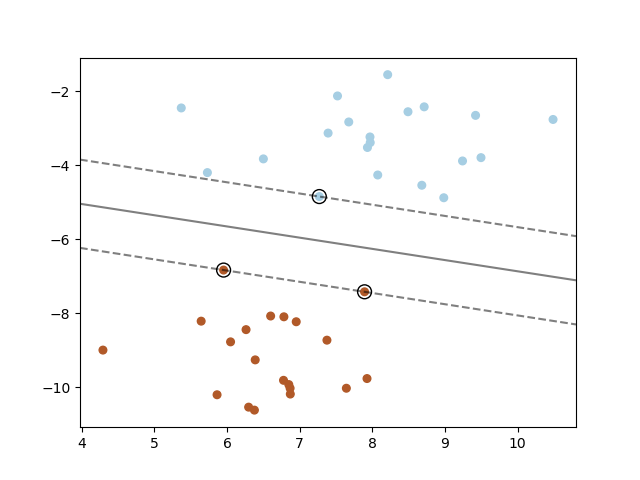
\includegraphics[width=.65\textwidth]{img/svm_hyperplane.png}
\caption{Esempio di iper-piano ricavato dall'apprendimento di un classificatore SVM per un problema di classificazione binario}
\label{img:svm_hyperplane}
\end{figure}

Per procedere con la selezione occorre trovare una regola con cui confrontare i risultati ottenuti. Il valore di controllo utilizzato è il valore di precisione nella classificazione LSVC usando l'intero set di feature. Per ottenere questo valore, il modello è stato addestrato e testato mediante cross-validation. Questa tecnica consiste in $N$ iterazioni dei seguenti passi:
\begin{enumerate}
    \item dato con un certo rapporto $\alpha \in (0,1)$, campionare il dataset $D$ per creare gli insiemi di training $D_{train}$ e test $D_{test}$ tale che $|D_{test}| = \alpha * |D|$ e $|D_{train}| = (1-\alpha) * |D|$.
    \item ad ogni iterazione, addestrare il classificatore con i campioni in $D_{train}$
    \item validare il modello appena creato utilizzando l'insieme di campioni in $D_{test}$
    \item misurare il valore di precisione $p_{i}$ del classificatore nell'${i}-esima$ iterazione.
\end{enumerate}

Il valore di precisione finale è dato da $\frac{1}{N} \sum_{i=1}^{N} p_{i}$.

Il campionamento avviene garantendo un dataset bilanciato ad ogni iterazione. Il rapporto utilizzato è $\alpha=0.2$. L'applicazione della cross-validation permette di limitare problemi di overfitting, ovvero la situazione in cui il modello perde di generalità e la precisione diminuisce quando usato per classificare esempi differenti \cite{arlot2010survey}.

Dato che la selezione è fatta separatamente per i due costrutti psicologici in esame, sono stati creati e addestrati due diversi classificatori per ottenere le precisioni di riferimento. Le feature da selezionare sono le 25 feature associate al costrutto e la variabile che si vuole predire è la media dei valori riportati nei questionari durante la sessione sperimentale.

Inoltre, per generalizzare meglio il modello, è stato cercato il coefficiente di regolarizzazione che fornisce la precisione più elevata. Variare il coefficiente di regolarizzazione implica variare la complessità del modello.

Il valore è stato cercato iterativamente: il modello è stato addestrato e testato variando coefficiente di regolarizzazione $C = 10^{-i}$, con $i\in(-10\dots+10)$. La figura \ref{img:regolarization_test} mostra l'andamento della precisione del classificatore al variare del coefficiente di regolarizzazione. I valori selezionati per valenza e arousal sono rispettivamente $1$ e $10^{-2}$

L'implementazione del classificatore è fornita dalla libreria LINEARSVM \cite{fan2008liblinear}.

\begin{figure}
\begin{tabular}{cc}
 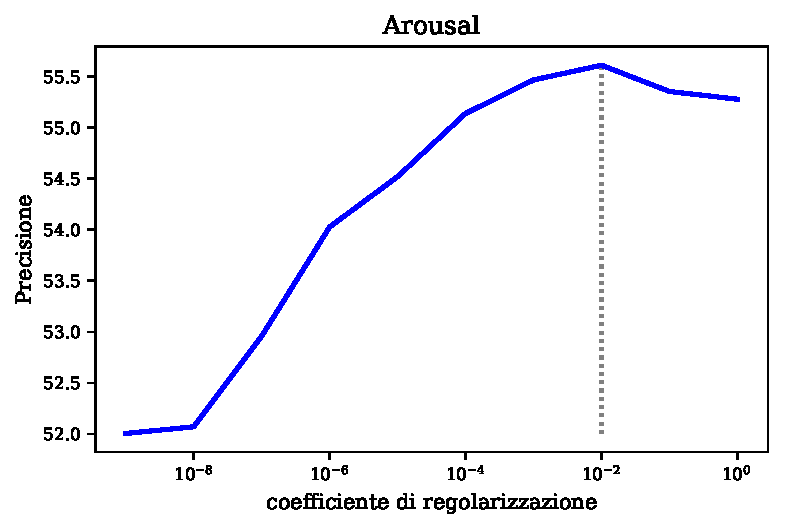
\includegraphics[width=.45\textwidth]{img/reg_coef_aro.pdf} & 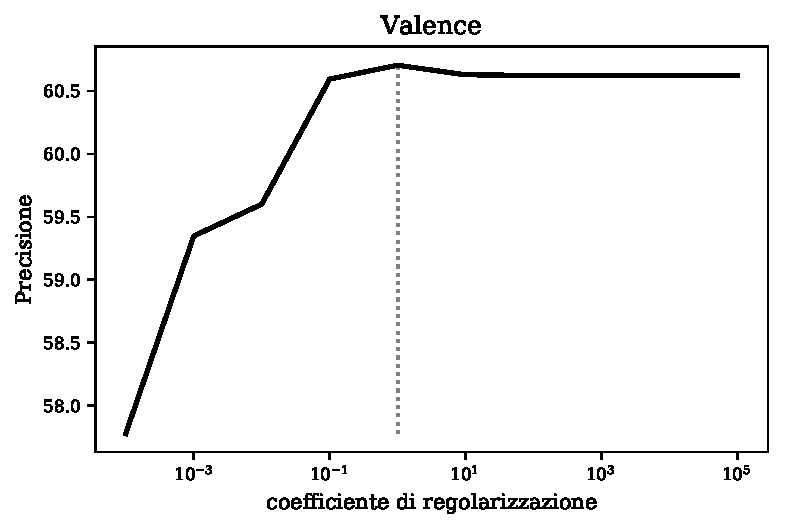
\includegraphics[width=.45\textwidth]{img/reg_coef_val.pdf}
\end{tabular}
\caption{Variazione della precisione di classificazione al variare del coefficiente di regolarizzazione. I valori ottimali sono indicati dalla linea verticale e sono rispettivamente $10^{-2}$ per l'arousal e $1$ per la valence}
\label{img:regolarization_test}
\end{figure}

In letteratura si distinguono due tipologie di metodi per la selezione delle feature: dato un insieme di feature $F$, i metodi $filter$ si basano su operazioni che filtrano le feature $f \in F$ meno rilevanti prima che il processo di classificazione avvenga. I metodi $wrapper$ generano un insieme di feature $F' \subseteq F$ che viene utilizzato per addestrare un classificatore e la sua accuratezza viene utilizzata come misura per valutare $F'$ rispetto ad $F$ \cite{langley1994selection}.

Un classificatore configurato con il parametro $C$ corretto è stato addestrato e testato considerando le feature selezionate automaticamente con le tecniche di seguito descritte.

\subsubsection*{$k$-best feature elimination ($kBest$)} è un metodo filter e la selezione si basa su test statistici applicati su feature e target. Successivamente, vengono conservate solo le $k$ feature che ottengono i miglior risultati. Il test utilizzato nella selezione è $F$-test. Ad ogni iterazione $i$, con $i \in (1, N)$ dove $N$ è il numero massimo di feature, viene selezionato un insieme di feature $F_{i}$, con $|F_{i}|=i$. Il classificatore viene addestrato con l'insieme di feature $F_{i}$ e valutato con cross-validazione. Il valore di precisione viene misurato come indice di efficacia dell'insieme $F_{i}$.

\subsubsection*{Recursive feature elimination con cross-validation ($RFECV$)} è un metodo wrapper, in \cite{weston2001feature} viene proposta una procedura iterativa in cui, per ogni passo di esecuzione $i$:
\begin{itemize}
  \item viene addestrato un classificatore con un insieme di feature $F_{i}$, tale che $|F_{i}| < |F_{i-1}|$
  \item viene applicato un criterio di valutazione e assegnato un valore di importanza ad ognuna delle feature $f \in F_{i}$. Ad esempio, può essere applicata la funzione $\phi(f) = w_{n}^2$ dove $w_{n}$ è il coefficiente che il classificatore lineare ha associato alla $n$-esima feature.
  \item viene rimossa la feature $f \in F_{i}$, tale che $\phi(f) = \min(\phi_{f_1}, \phi_{f_2}, \dots, \phi_{f_n})$
\end{itemize}

Al termine della processo sono state selezionate 23 feature per valence e 4 per arousal. I coefficienti attribuiti dal classificatore SVM relativo alla selezione sono stati salvati per le fasi successive.

\subsection{Gaze Heatmap}

Le heatmap sono rappresentazioni grafiche di una variabile di interesse, i cui valori, contenuti in una matrice, sono mappati in un certo schema colori. Nel caso delle gaze heatmap quindi, viene rappresentata la distribuzione nello spazio dei punti di fissazione di uno o più soggetti.

La creazione di una heatmap può essere schematizzata in tre fasi: accumulazione, normalizzazione e colorazione.

\subsubsection*{Accumulazione}
Presa una immagine $P$ di dimensione $m$ x $n$, composta da pixel $p_{i,j}$ di coordinate $(i,j)$, definiamo la matrice di heatmap $H$, i cui elementi $h_{i,j}$ rappresentano il valore di heatmap per il pixel $p_{i,j}$. Tenendo presente che il gaze tracker fornisce le coordinate delle fissazioni $(x,y)$ proiettate nello spazio coordinate dell'immagine target, definiamo $f_{x,y} \in F$ il punto di fissazione nelle coordinate $(x,y)$ con $x \in (0,m)$ e $y \in (0,n)$.

Per ogni $f_{x,y} \in F$, per ogni pixel $h_{i,j} \in H$ viene assegnato un valore di intensità $I$ secondo la relazione:

\begin{equation}
  I(h_{i,j}) = s(f_{x,y} ,h_{i,j}) * w(f_{x,y})
  \label{eq:heatmap_intensity}
\end{equation}

dove, $s$ è una funzione di scalatura e $w$ è una funzione che assegna un peso per la specifica fissazione.

La funzione $s$ rappresenta la probabilità che il pixel $h_{i,j} = p_{i,j}$ venga osservato durante la fissazione $f_{x,y}$ ed è stata modellata secondo la distribuzione Gaussiana:

\begin{equation}
  s = e^{\frac{-((x-i)^2+(y-j)^2)}{2\sigma^{2}}}
\end{equation}

La costante $\sigma$ è espressa in termini di \textit{Full Width at Half Maximum} (FWHM). Anche se in \cite{wooding2002eye} viene fatto notare che la larghezza della distribuzione Gaussiana corretta dovrebbe dipendere dal task cui è sottoposto il soggetto, \cite{blignaut2010visual} consiglia di definire FWHM per rappresentare il 40\% dell'angolo massimo di visuale parafoveale $\theta$:

\begin{equation}
  \sigma = 0.17 x \theta
\end{equation}

dove $\theta$ è funzione della distanza del soggetto dallo schermo e rappresenta il numero di pixel osservati considerando un angolo di visuale di 5°.

La funzione $w$ rappresenta la metrica utilizzata per calcolare l'intensità, e generalmente se ne utilizza una tra numero di fissazioni, durata assoluta delle fissazioni, durata relativa delle fissazioni e numero di partecipanti. Per il calcolo delle gaze heatmap è stata utilizzata la durata assoluta delle fissazione fornita direttamente dal database utilizzato.

\subsubsection*{Normalizzazione}
Per poter confrontare le heatmap occorre applicare una normalizzazione prima della fase di colorazione. I valori delle heatmap $H$ sono stati scalati in un range [0,1] applicando la normalizzazione min-max, ottenendo una nuova heatmap $H'$ come:

\begin{equation}
  H'_{i,j} = \frac{H_{i,j}-{H_{min}}}{H_{max}-H_{min}}
  \label{eq:min_max_normalization}
\end{equation}

per ogni pixel in $i,j \in H$.

\subsubsection*{Colorazione}
Le gaze heatmap possono essere colorate utilizzando diversi modelli basati su variazioni di luminanza e variazioni cromatiche.
In \cite{pomplun1996disambiguating}, le heatmap sono state rappresentate sovrapponendo all'immagine di riferimento una maschera in grado di variare il livello di luminosità, mettendo in risalto le porzioni di immagine più osservate.
Nelle heatmap più moderne vengono utilizzati i gradienti di colore anche se in \cite{borland2007rainbow} è stato dimostrato che questi presentano alcuni difetti, come ad esempio la mancanza implicita di un ordine percettivo nelle differenze di tonalità.
In questo lavoro viene utilizzato il gradiente colore \textit{Jet}, che varia tra tonalità di blu per aree con poche fissazioni e con il rosso per aree con molte fissazioni.

\subsection{Heatmap Fisiologiche}

Nelle heatmap fisiologiche, l'equazione di intensità \ref{eq:heatmap_intensity} rappresenta l'intensità della risposta fisiologica del soggetto durante una specifica fissazione. La funzione di peso $w$ va quindi modificata per tenere in considerazione i segnali fisiologici. Le heatmap sono state generate considerando i costrutti psicologici separatamente, ottenendo così heatmap di valenza e heatmap di arousal. I segnali fisiologici utilizzati nella generazione delle due diverse mappe sono quelli selezionati mediante il processo descritto nella sezione \ref{section:feature_selection}.

I coefficienti assegnati dai classificatori SVM durante la fase di selezione sono stati scalati in modo tale che $\sum_{n=1}^{N} \phi(f_{n}) = 1$ con $N$ numero di feature selezionato per il costrutto psicologico. I coefficienti scalati sono considerati come la probabilità che una certa feature partecipi alla generazione della heatmap fisiologica.

La funzione di peso $w$ è trasformata per rappresentare il valore di risposta fisiologica pesata per ogni feature durante la fissazione nelle coordinate (x,y), e si può definire come combinazione lineare dalla relazione:

\begin{equation}
  w(f_{x,y}) = \sum_{n=1}^{N}\phi(f_{n})*f_{n}(x,y)
\end{equation}

Le heatmap generate sono state normalizzate e il criterio di soglia introdotto nella sezione precedente è stato utilizzato per filtrare le aree interessate da una minore risposta fisiologica.

